\section{Loading Spinners}
\label{prototype:LoadingSpinner}
Loading spinners are a common UI element used to indicate that a process is ongoing, such as data loading or processing. They provide visual feedback to users, helping them understand that the application is working on their request whilst minimising the percieved wait time. 

In keeping with my application design principles, I have designed a loading spinner that is both visually appealing and functional.

\begin{figure}[H]
    \centering
    \begin{subfigure}[b]{0.45\textwidth}
        \centering
        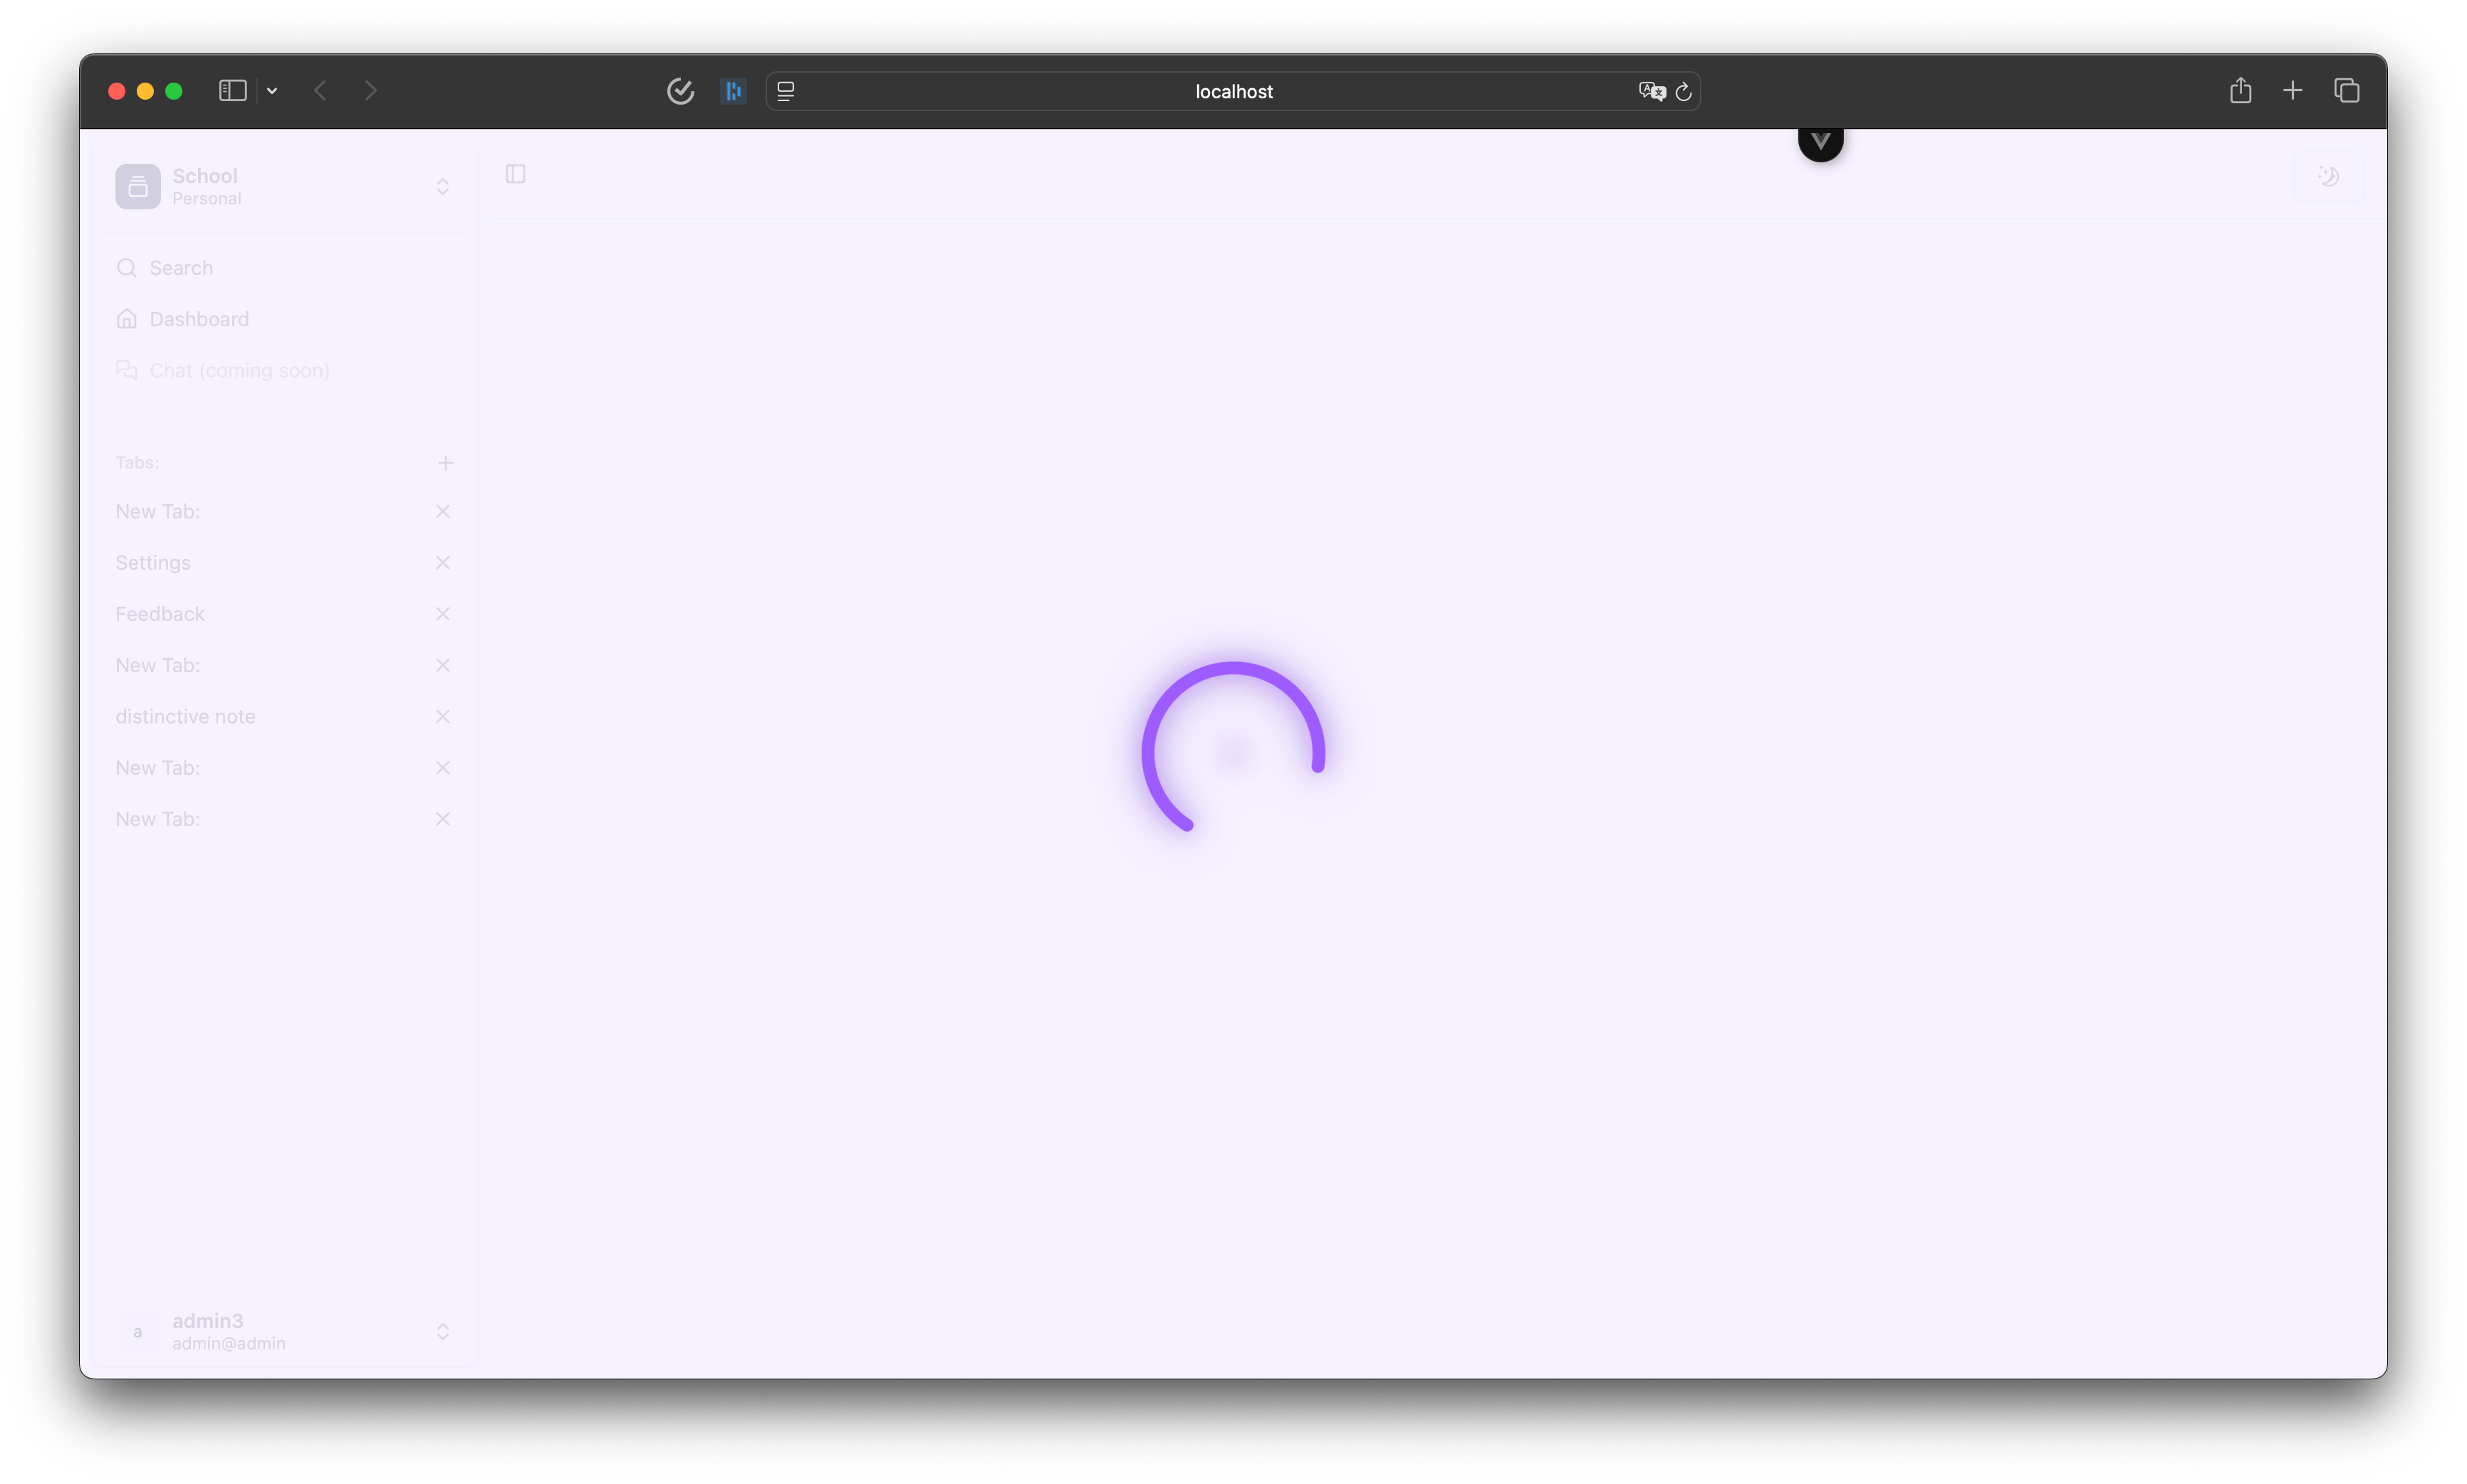
\includegraphics[width=\textwidth]{Prototype/22_LoadingSpinner/media/lightSpinner.png}
        \caption{Light mode}
    \end{subfigure}
    \hfill
    \begin{subfigure}[b]{0.45\textwidth}
        \centering
        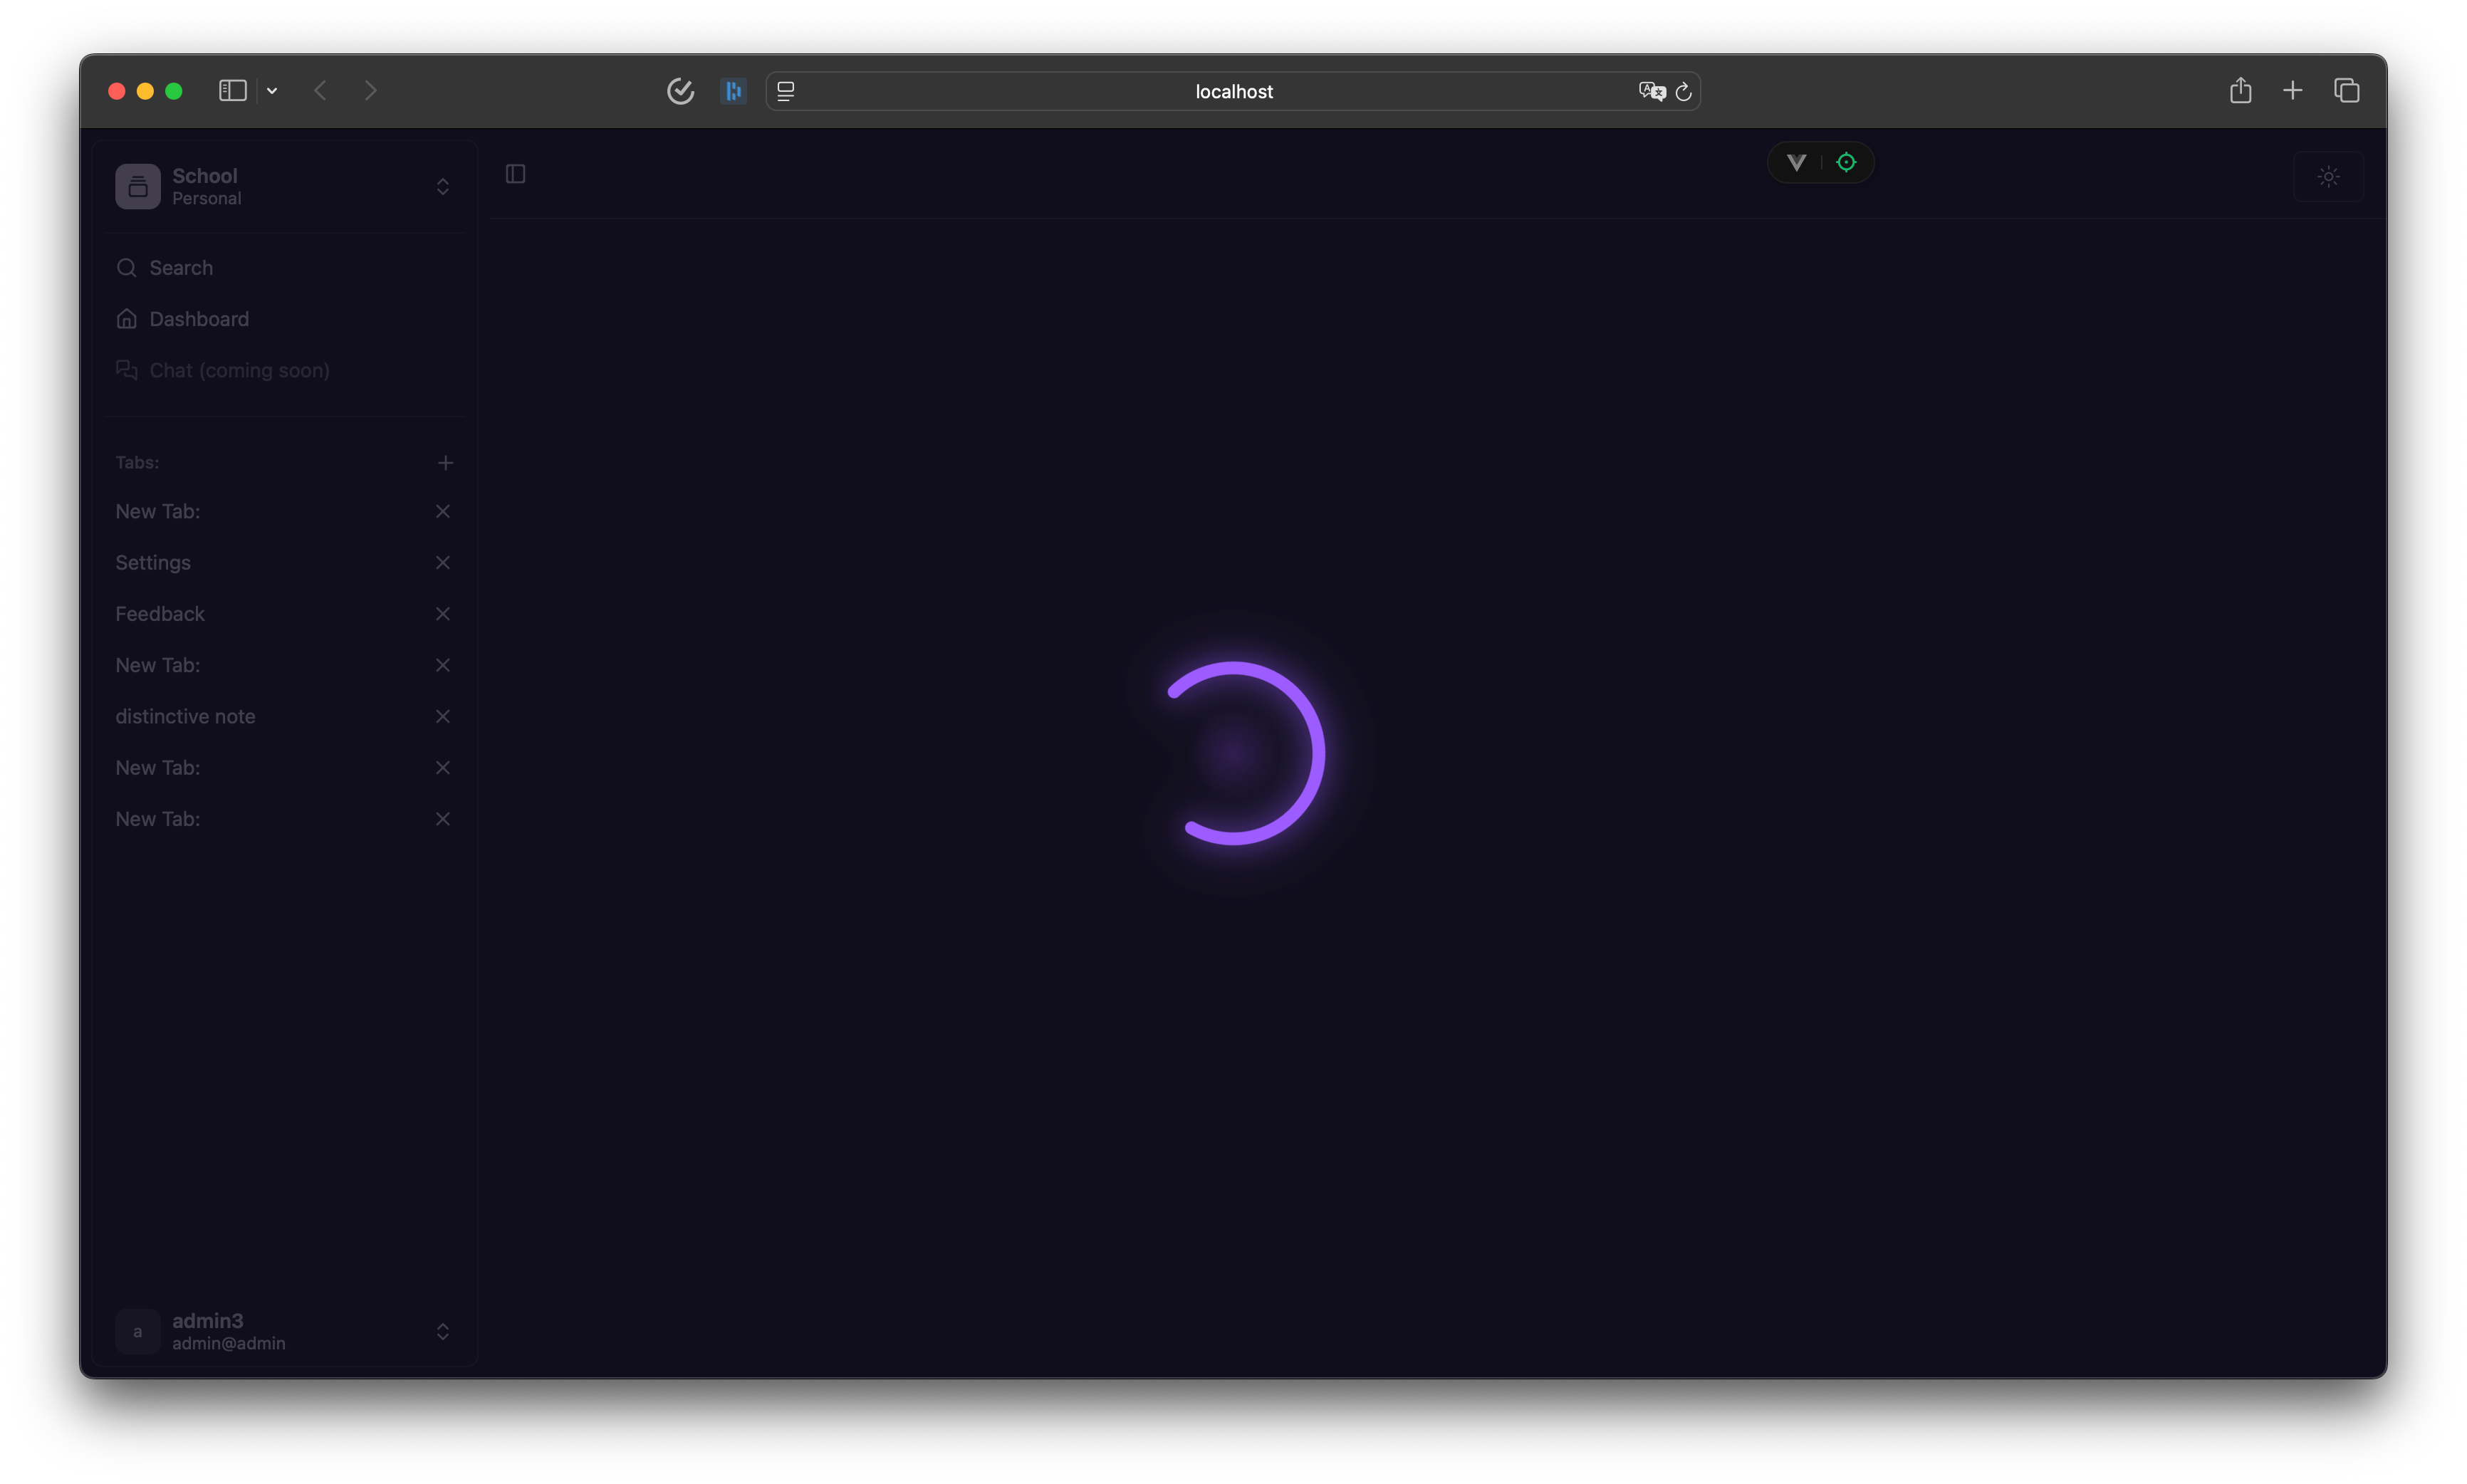
\includegraphics[width=\textwidth]{Prototype/22_LoadingSpinner/media/darkSpinner.png}
        \caption{Dark mode}
    \end{subfigure}
    \caption{The Loading Spinner in light and dark mode.}
\end{figure}